Here's some TikZ code that creates the two shapes you described:
```
\documentclass{standalone}
\usepackage{tikz}
\begin{document}
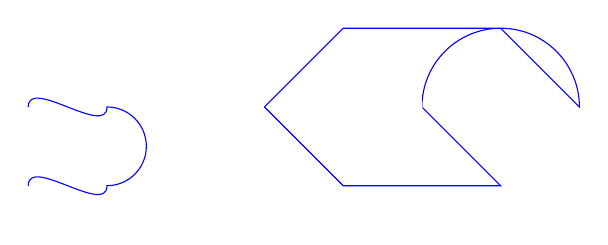
\begin{tikzpicture}
  % Left shape: modified curve with circular ends
  \draw[blue] (0,0) to[out=90,in=270] ++(1,0)
              arc[start angle=90,end angle=-90,radius=0.5]
              to[out=270,in=90] ++(-1,0);
  
  % Right shape: mix of curves and lines, with cut-out circle in the center
  \draw[blue] (3,0) -- (4,1) -- (6,1) -- (7,0)
              arc[start angle=0,end angle=180,radius=1]
              -- (6,-1) -- (4,-1) -- (3,0);
  \filldraw[white] (4.5,0) circle[radius=0.5];
\end{tikzpicture}
\end{document}
```
This code creates two blue shapes side by side. The left shape is a modified curve with circular ends, created using the `to` command with custom angles for the curves and the `arc` command for the circular ends. The right shape is a mix of curves and lines, with a cut-out circle in the center. The circle is drawn using the `filldraw` command with a white fill color to make it appear as a cut-out.